\documentclass[12pt]{article}
\usepackage{amsmath}
\usepackage{amsfonts}
\usepackage{amssymb}
\usepackage{hyperref}
\usepackage{graphicx}

\title{Numerical Relativity Project: Geodesics Around a Massive Body}
\author{Your Name}
\date{\today}

\begin{document}

\maketitle

\tableofcontents

\newpage

\section*{Introduction}

In this project, we simulate the interaction between a small mass orbiting a large mass using numerical relativity techniques. The goal is to visualize the geodesics in the spacetime field around the large mass and analyze the interaction between the two masses. The project is divided into the following steps:
\begin{enumerate}
    \item Define the problem framework.
    \item Set up the geodesic equations.
    \item Implement numerical methods for solving the equations.
    \item Visualize the results to interpret the dynamics.
    \item Represent the spacetime field to complement the geodesic visualization.
\end{enumerate}

Each step is detailed in its respective chapter, including Python code and mathematical derivations.

\newpage

\section{Defining the Problem Framework}

In this chapter, we define the Schwarzschild metric, which describes spacetime around a non-rotating, spherically symmetric massive body. The metric is given by:
\[
ds^2 = -\left(1 - \frac{2M}{r}\right)dt^2 + \left(1 - \frac{2M}{r}\right)^{-1}dr^2 + r^2 \left(d\theta^2 + \sin^2\theta \, d\phi^2 \right)
\]

Here, \(M\) is the mass of the central body, and \(r, \theta, \phi\) are spherical coordinates. The metric coefficients \(g_{\mu\nu}\) are:
\[
g_{\mu\nu} = 
\begin{pmatrix}
-\left(1 - \frac{2M}{r}\right) & 0 & 0 & 0 \\
0 & \left(1 - \frac{2M}{r}\right)^{-1} & 0 & 0 \\
0 & 0 & r^2 & 0 \\
0 & 0 & 0 & r^2 \sin^2\theta
\end{pmatrix}
\]

We derive the Christoffel symbols using the metric coefficients:
\[
\Gamma^\lambda_{\mu\nu} = \frac{1}{2} g^{\lambda\rho} \left( \frac{\partial g_{\rho\mu}}{\partial x^\nu} + \frac{\partial g_{\rho\nu}}{\partial x^\mu} - \frac{\partial g_{\mu\nu}}{\partial x^\rho} \right)
\]

These symbols are essential for formulating the geodesic equations.

\newpage

\section{Setting Up the Geodesic Equations}

To compute the motion of the small mass in the spacetime described by the Schwarzschild metric, we use the geodesic equations:
\[
\frac{d^2 x^\mu}{d\tau^2} + \Gamma^\mu_{\nu\lambda} \frac{dx^\nu}{d\tau} \frac{dx^\lambda}{d\tau} = 0
\]

Here, \(x^\mu = (t, r, \theta, \phi)\) represents the coordinates of the particle, \(\tau\) is the proper time, and \(\Gamma^\mu_{\nu\lambda}\) are the Christoffel symbols of the Schwarzschild metric.

To solve these equations numerically, we convert them into a system of first-order differential equations by introducing the velocity components:
\[
v^\mu = \frac{dx^\mu}{d\tau}
\]

The system then becomes:
\[
\frac{dx^\mu}{d\tau} = v^\mu, \quad \frac{dv^\mu}{d\tau} = -\Gamma^\mu_{\nu\lambda} v^\nu v^\lambda
\]

This formulation allows us to solve the equations using numerical methods.

\newpage

\section{Numerical Integration of Geodesics}

To solve the geodesic equations derived in Chapter 2, we use numerical methods. Specifically, we employ a Runge-Kutta method provided by \texttt{scipy.integrate.solve\_ivp} in Python. This solver computes the trajectory of a small mass in the Schwarzschild spacetime by integrating the equations:
\[
\frac{dx^\mu}{d\tau} = v^\mu, \quad \frac{dv^\mu}{d\tau} = -\Gamma^\mu_{\nu\lambda} v^\nu v^\lambda
\]

The solver requires:
\begin{itemize}
    \item Initial conditions for the position \(x^\mu = (t, r, \theta, \phi)\) and velocity \(v^\mu\).
    \item The proper time interval \(\tau\) over which to integrate.
\end{itemize}

The results of the integration are stored as trajectories for visualization in subsequent chapters.

\newpage

\section{Visualization of Geodesics}

The geodesics computed in Chapter 3 are visualized to understand the motion of the small mass in the Schwarzschild spacetime. The visualization includes:
\begin{itemize}
    \item A 2D projection of the trajectory in the equatorial plane (\(x-y\)).
    \item A 3D visualization of the geodesics to capture the full motion.
    \item An optional embedding diagram to show the spacetime curvature.
\end{itemize}

The trajectory is computed in spherical coordinates \((r, \theta, \phi)\) and converted to Cartesian coordinates for plotting:
\[
x = r \sin\theta \cos\phi, \quad y = r \sin\theta \sin\phi, \quad z = r \cos\theta
\]

These visualizations provide an intuitive representation of the dynamics.

\newpage

\section{Representation of the Spacetime Field}

In this chapter, we compute and visualize the curvature of the Schwarzschild spacetime. Curvature is characterized by quantities derived from the metric tensor, such as:
\begin{itemize}
    \item The Riemann curvature tensor \(R^\rho_{\sigma\mu\nu}\),
    \item The Ricci curvature tensor \(R_{\mu\nu}\),
    \item The Kretschmann scalar \(K = R^{\rho\sigma\mu\nu} R_{\rho\sigma\mu\nu}\).
\end{itemize}

The Schwarzschild spacetime is vacuum, so the Ricci tensor vanishes (\(R_{\mu\nu} = 0\)). The Kretschmann scalar is given by:
\[
K = \frac{48M^2}{r^6}
\]
which represents the intensity of spacetime curvature. It diverges as \(r \to 0\), indicating the singularity at the center.

The field is visualized as a scalar field \(K(r)\) overlayed on the geodesics to illustrate the relationship between curvature and motion.

\begin{figure}[h]
    \centering
    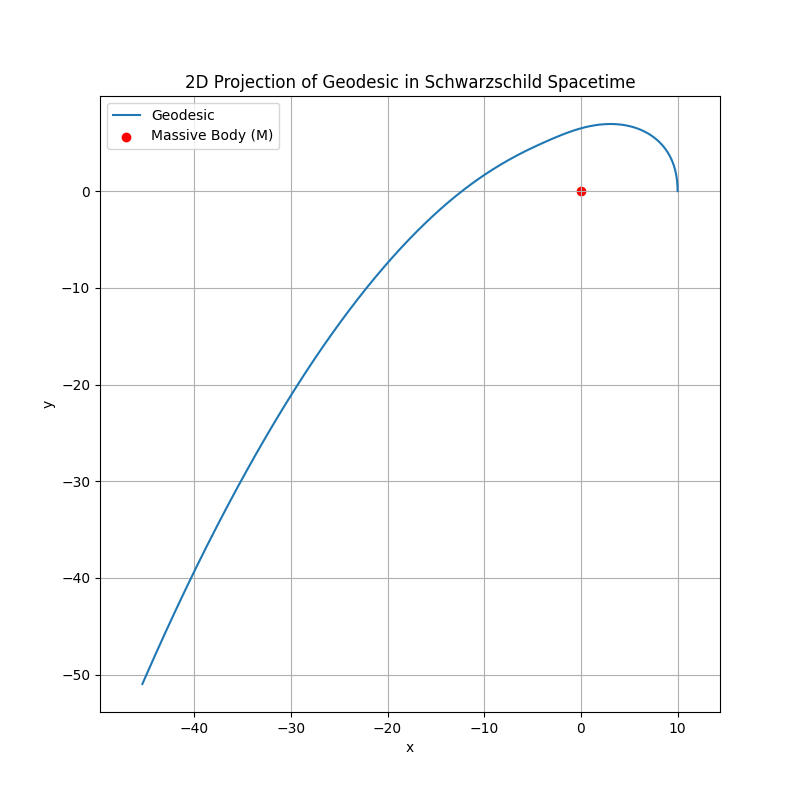
\includegraphics[width=0.8\textwidth]{geodesic_2d_projection.png}
    \caption{2D Projection of Geodesic in Schwarzschild Spacetime.}
    \label{fig:2d_projection}
\end{figure}

\begin{figure}[h]
    \centering
    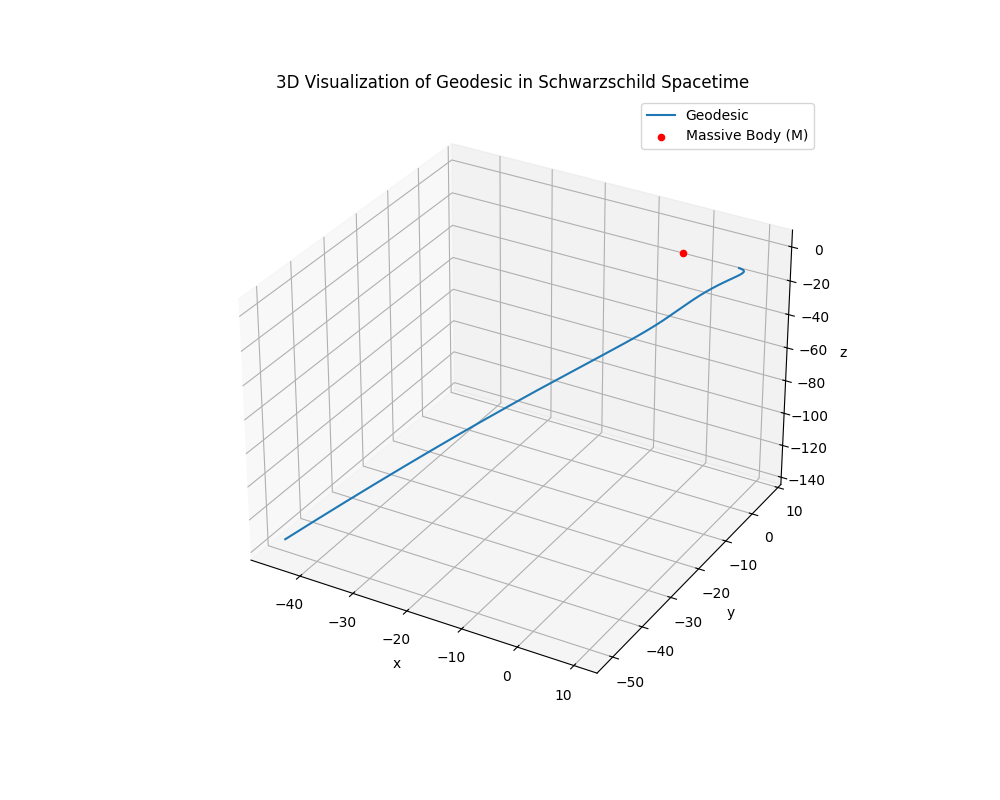
\includegraphics[width=0.8\textwidth]{geodesic_3d_trajectory.png}
    \caption{3D Visualization of Geodesic in Schwarzschild Spacetime.}
    \label{fig:3d_trajectory}
\end{figure}

\begin{figure}[h]
    \centering
    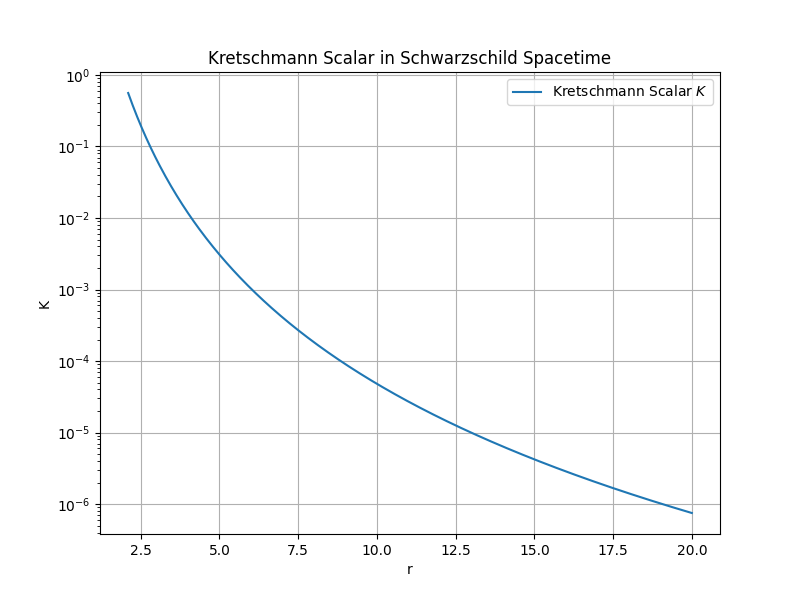
\includegraphics[width=0.8\textwidth]{kretschmann_scalar.png}
    \caption{Kretschmann Scalar as a Function of Radial Distance.}
    \label{fig:kretschmann_scalar}
\end{figure}

\begin{figure}[h]
    \centering
    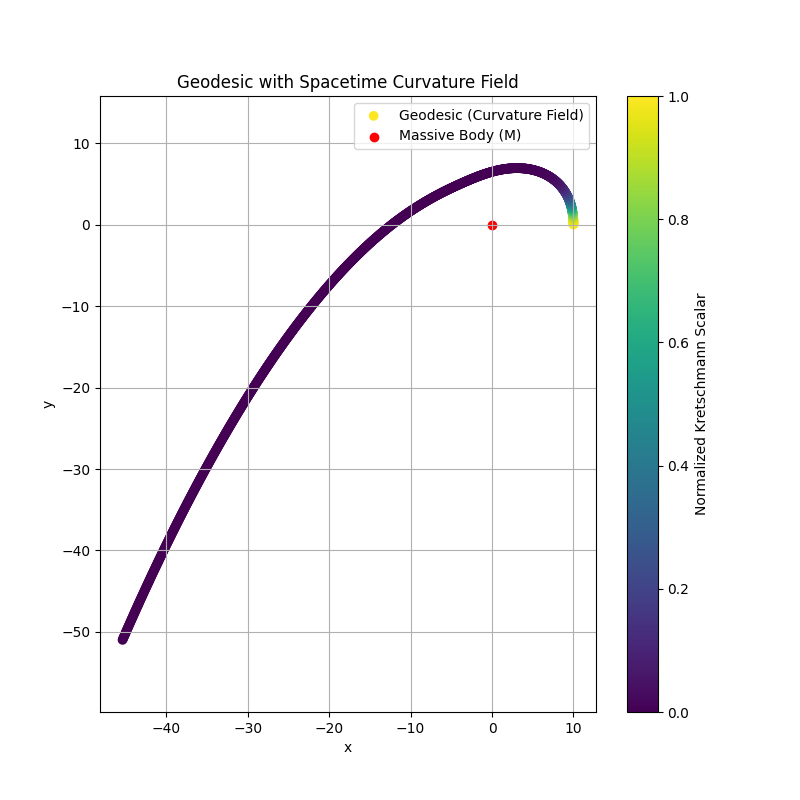
\includegraphics[width=0.8\textwidth]{geodesic_curvature_field.png}
    \caption{Geodesic with Normalized Spacetime Curvature Field Overlay.}
    \label{fig:curvature_field}
\end{figure}


\end{document}
